% Autor: Dominik Harmim <xharmi00@stud.fit.vutbr.cz>


\documentclass[a4paper, 11pt, twocolumn]{article}


\usepackage[czech]{babel}
\usepackage[utf8]{inputenc}
\usepackage[left=2cm, top=2cm, text={17cm, 25cm}]{geometry}
\usepackage{times}
\usepackage{graphicx}
\usepackage[unicode, colorlinks, hypertexnames=false, citecolor=red]{hyperref}


\begin{document}
	%%%%%%%%%%%%%%%%%%%%%%%%%%%%%%%% Titulek %%%%%%%%%%%%%%%%%%%%%%%%%%%%%%%%%%%
	\twocolumn[
		\begin{@twocolumnfalse}
			\begin{center}
				{\Large
					Vysoké učení technické v~Brně \\
					Fakulta informačních technologií \\
				}
				{
\includegraphics[width=0.4 \linewidth]{inc/FIT_logo.pdf}} \\

				{\LARGE
					Mikroprocesorové a~vestavěné systémy \\
					Projekt\,--\,Měření srdečního tepu \\[0.4cm]
				}

				{\large
					Dominik Harmim (xharmi00) \\
					\texttt{xharmi00@stud.fit.vutbr.cz} \\
					\today
				}
			\end{center}
		\end{@twocolumnfalse}
	]



	%%%%%%%%%%%%%%%%%%%%%%%%%%%%%%%% Úvod %%%%%%%%%%%%%%%%%%%%%%%%%%%%%%%%%%%%%%
	\section{Úvod}

	Zadáním projektu byl návrh a~implementace vestavné aplikace na výukové
	desce FitKit~3 \cite{fitkit}, která obsahuje mikrokontrolér
	MCU Freescale KINETIS (MK60DN512ZVMD10), viz manuál \cite{k60_manual}.
	K~této desce se připojí modul pro měření srdečního tepu a~modul se
	segmentovým LED displejem (zapojení těchto součástek bylo taktéž
	součástí řešní). Výsledná aplikace bude měřit frekvenci srdečního
	tepu (počet tepů za minutu) a~bude zobrazovat výsledek na LED
	displeji.

	Vestavná aplikace byla implementována v~jazyce C~v~prostředí
	MCUXpresso IDE s~využitím SDK pro MCU K60 \cite{sdk}.



	%%%%%%%%%%%%%%%%%%%%%%%%%%%%%%%% Zapojení hardware %%%%%%%%%%%%%%%%%%%%%%%%%
	\section{Zapojení hardware}

	Všechny externí moduly byly k~desce FitKit~3 připojeny na skupinu
	pinů označených P1 (viz schéma zapojení FitKit~3 \cite{fitkit_schema}).


	\subsection {Modul pro měření srdečního tepu}

	Modul pro měření srdečního tepu obsahuje tři vývody: napájení (+\,3,3\,V),
	uzemění a~analogový výstup, jak demonstruje obrázek \ref{fig:sensor}.
	Napájení bylo zapojeno na pin č.~1, uzemění na pin č.~49 a~analogový
	výstup na pin č.~14. Toto zapojení je znázorněno na obrázku
	\ref{fig:hardware_connection}.

	\begin{figure}[ht]
		\centering
		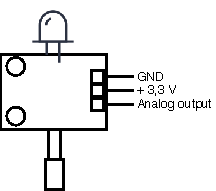
\includegraphics[width=0.8 \linewidth]{inc/sensor.pdf}

		\caption{Modul pro měření srdečního tepu}
		\label{fig:sensor}
	\end{figure}


	\subsection{Modul se segmentovým displejem}

	Modul se segmentovým displejem obsahuje čtyři číslice skládající se ze
	sedmi segmenů standardně označených A-G a~desetinnou tečkou za každou
	z~číslic standardně označenou jako DP. Modul obsahuje 8 vstupních pinů
	pro aktivaci těchto segmentů, včetně destinné tečky. Modul obsahuje další
	čtyři vstupní piny pro aktivaci jednotlivých číslic. Tyto piny jsou
	označeny C1-C4. V~jednu chvíli může být aktivní pouze jedna číslice.
	Všechny výše uvedené piny jsou umístěny ve skupině pinů JP1 na zadní
	straně modulu. Význam jednotlivých pinů je uveden na obrázku
	\ref{fig:display}. Skipina pinů JP1 byla zapojena na piny 17-28.
	Toto zapojení je naznačeno na obrázku \ref{fig:hardware_connection}.

	\begin{figure}[ht]
		\centering
		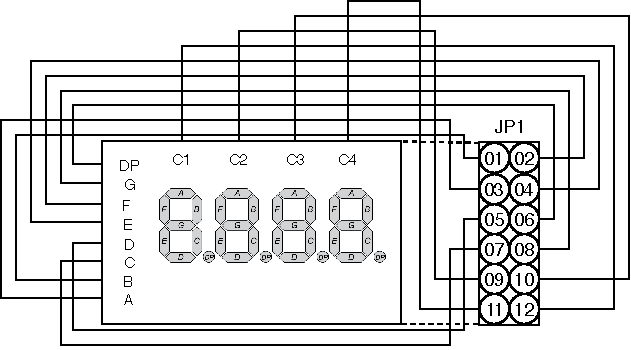
\includegraphics[width=1 \linewidth]{inc/display.pdf}

		\caption{Modul se segmentovým displejem}
		\label{fig:display}
	\end{figure}

	\begin{figure}[ht]
		\centering
		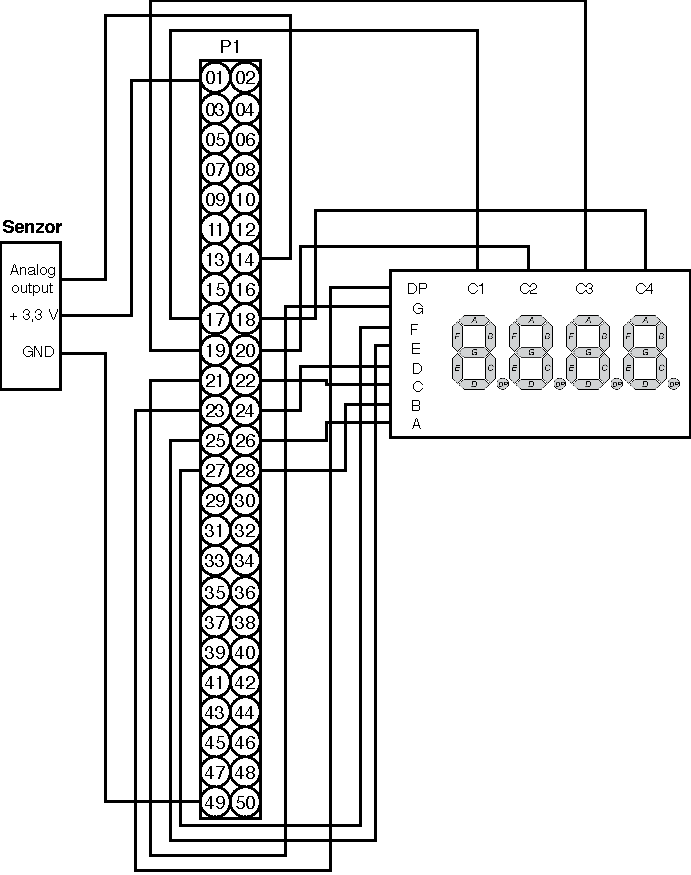
\includegraphics[width=1 \linewidth]{inc/hardware_connection.pdf}

		\caption{Schéma zapojení}
		\label{fig:hardware_connection}
	\end{figure}


	\subsection{Význam zapojení}

	Význam jednotlivých pinů a~jejich použití v~MCU, na které byly zapojeny
	výše uvedené moduly je popsán v~tabulce \ref{tab:hardware_connection}.

	\begin{table}[ht]
		\centering
		\begin{tabular}{p{1.3cm} p{1.3cm} p{1.2cm} p{2.2cm}}
			\hline
			Pin & Zapojení na desce & Označení v~MCU & Použití v~MCU \\ \hline
			Senzor & P1\,--\,14 & L1 & ADC0 CH0~P \\
			Disp~A & P1\,--\,26 & L9 & PTA11 \\
			Disp~B & P1\,--\,28 & L8 & PTA9 \\
			Disp~C & P1\,--\,22 & C2 & PTD14 \\
			Disp~D & P1\,--\,24 & M9 & PTA10 \\
			Disp~E & P1\,--\,25 & J7 & PTA6 \\
			Disp~F & P1\,--\,27 & J8 & PTA7 \\
			Disp~G & P1\,--\,21 & C1 & PTD15 \\
			Disp DP & P1\,--\,23 & K8 & PTA8 \\
			Disp C1 & P1\,--\,17 & C9 & PTD8 \\
			Disp C2 & P1\,--\,20 & C3 & PTD13 \\
			Disp C3 & P1\,--\,19 & B1 & PTD12 \\
			Disp C4 & P1\,--\,18 & B9 & PTD9 \\ \hline
		\end{tabular}

		\caption{Význam zapojení}
		\label{tab:hardware_connection}
	\end{table}



	%%%%%%%%%%%%%%%%%%%%%%%%%%%%%%%% Způsob řešení %%%%%%%%%%%%%%%%%%%%%%%%%
	\section{Způsob řešení}

	Implementace se nachází v~souborech v~adresářích \texttt{board}
	a~\texttt{source}. Ostatní soubory byly vygenerovány při vytvoření
	projektu pro MCU K60 v~prostředí MCUXpresso IDE.

	V~projektu jsou přímo využívány následující komponenty SDK pro MCU K60
	(jsou umístěny v~adresáři \texttt{drivers}):
	\begin{itemize}
		\item
			\textbf{ADC16} (16-bit SAR Analog-to-Digital Converter
			Driver)\,--\,čtení analogového signálu ze senzoru serdečního tepu
			a~jeho převod do digitální podoby.

		\item
			\textbf{CLOCK} (Clock Driver)\,--\,nastavování hodin.

		\item
			\textbf{GPIO} (General-Purpose Input/Output Driver)\,--\,nastavování
			vstupních a~výstupních pinů a~zápis na vstupní piny LED
			displeje.

		\item
			\textbf{LPTMR} (Low Power Timer Driver)\,--\,počítání času měření
			srdečního tepu a~času mezi jednotlivými srdečními pulsy.

		\item
			\textbf{PIT} (Periodic Interrupt Timer Driver)\,--\,periodické
			obnovování LED displeje.

		\item
			\textbf{PORT} (Port Control and Interrupts)\,--\,nastavování
			vstupních a~výstupních portů.
	\end{itemize}

	Vstupní bod aplikace (funkce \texttt{main}) se nachází v~soubobru
	\texttt{source/main.c}. Na začátku programu proběhne inicializace
	hardware a~následně v~nekonečné smyčce probíhá měření srdečního tepu
	a~zobrazování tepové frekvence na displej.


	\subsection{Konfigurace pinů}

	Konfiguraci vstupních a~výstupních pinů byla nastavena v~nástroji
	v~prostředí MCUXpresso IDE, který na základě této konfigurace vytvořil
	soubory \texttt{board/pin\_mux.h} a~\texttt{board/pin\_mux.c}. Tento nástroj
	k~tomuto nastavení používá funkce komponent \texttt{GPIO} a~\texttt{PORT}.


	\subsection{Segmentový LED displej}

	Na začátku běhu aplikace se provádí inicializace časovače \texttt{PIT},
	který periodicky v~pravidelných intervalech zobrazuje jednotlivé číslice
	na LED displeji. Každých 4\,166\,$ \mu $s se generuje přerušení, které
	zobrazí další číslici. Toto odpovídá obnovovací frekvenci 60\,Hz celého
	displeje. Nastavování jednotlivých pinů displeje se dělá funkcemi
	komponenty \texttt{GPIO}. Implementace displeje se nachází v~souborech
	\texttt{source/display.h} a~\texttt{source/display.c}.


	\subsection{Měření srdečního tepu}

	Na začátku běhu aplikace se provádí inicializace časovače \texttt{LPTMR},
	který je použit pro měření času mezi jednotlivými měřeními srdečního tepu
	a~času mezi jednotlivými srdečními impulsy. Tento časovač je vynulován
	při každém novém měření. Dále se provádí inicializace analogově-digitálního
	převodníku \texttt{ADC16}, který se používá pro čtení signálu ze senzoru
	a~jeho převodu do digitální podoby. Samotný výpočet tepové frekvence je
	implementován v~souborech \texttt{source/sensor.h}
	a~\texttt{source/sensor.c}.

	Po přečtení signálu ze senzoru srdečního tepu funkcemi komponenty
	\texttt{ADC16} se signál filtruje. Provádí se tzv. dolní propust
	\cite{low_pass_filter}, která v~signálu potlačí vyšší frekvence, tzn.
	bude odstraněn šum na vyšších frekvencích. Následně se provádí tzv.
	horní propust \cite{high_pass_filter}, která v~signálu potlačí
	nižší frekvence, tzn. signál se bude pohyboval okolo nuly. Již filtrovaný
	signál je ilustrován na obrázku \ref{fig:sensor_data}.

	Vždy, když signál v~nejvyšším bodě začně klesat, je detekován srdeční
	impuls. Počet srdečních tepů za jednu minutu je vypočítán vztahem
	$ rate = \frac{60}{t} $, kde proměnná $ t $~je čas mezi dvěma impulsy.
	Tímto způsobem je zprůměrováno pět po sobě jdoucích hodnot a~výsledek
	je zobrazen na LED displej. Navíc je každý nový výsledek průměrovách
	i~s~několika předchozími, takže pokud je na senzoru přiložený prst
	delší dobu, tak by zobrazovaná tepová frekvence měla konvergovat
	k~přesnějším výsledkům. Měření tepové frekvence je restartováno pár
	sekund po odejmutí prstu ze senzoru.

	\begin{figure}[ht]
		\centering
		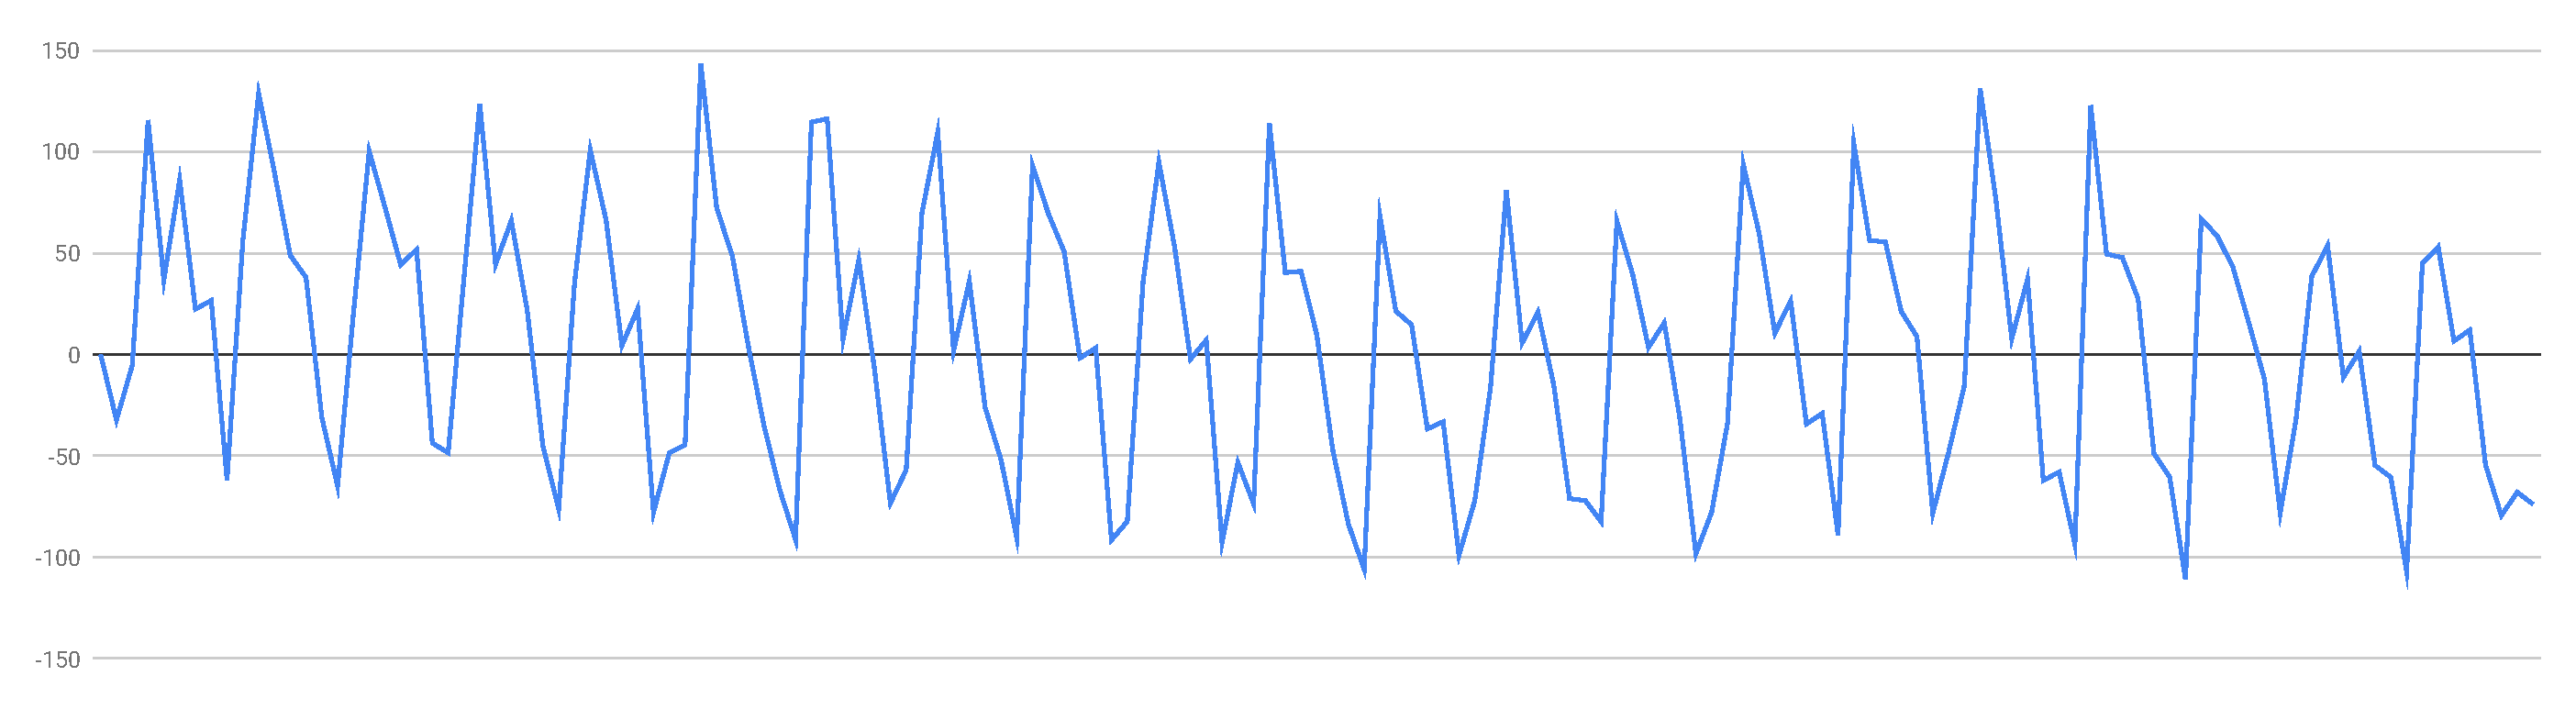
\includegraphics[width=1 \linewidth]{inc/sensor_data.pdf}

		\caption{Signál ze senzoru srdečního tepu}
		\label{fig:sensor_data}
	\end{figure}


	\section{Závěr}

	V~projektu se podařilo implementovat všechny body zadání. Řešení je
	v~zásadě funkční, pouze je potřeba dát si pozor na to, jak je vzdálená
	dioda od senzoru u~modulu pro měření tepu a~taky je nutné s~prstem na
	senzoru co nejméně pohybovat v~průběhu měření, v~opačném případě naměřené
	hodnoty nemusí odpovídat skutečnosti. Při testování implementace jsem
	naměřené výsledky porovnával s~naměřenými výsledky ze sportovních
	chytrých hodinek Xiaomi Amazfit Pace. Při testování za ideálních podmínek
	se naměřené hodnoty lišily jen nepatrně.



	%%%%%%%%%%%%%%%%%%%%%%%%%%%%%%%% Citace %%%%%%%%%%%%%%%%%%%%%%%%%%%%%%%%%%%%
	\bibliographystyle{czechiso}
	\renewcommand{\refname}{Literatura}
	\bibliography{documentation}
\end{document}
